\chapter{Design}

The goal of this chapter is to outline and discuss the overall architecture and design of the system, including the major components, their area of responsibility, and how they fit together. Additionally, a short discussion about the changes and simplifications the design have endured during development, and why these changes were made.

\section{Architecture}

The overall architecture is based heavily on microservice principles, RESTful services, and ephemeral, stateless component instances. There is a single outlier to this in one particular component, the Media Relay Server, which is closer to a simpler client-server design. The primary driver for the choice of architecture is the need for the system to be easily horizontally scalable, as well as to be deployed through containerization technologies, in particular Kubernetes, which works well with such designs, as well as further provide reliability through redundancy.

\section{Design}

The system design is composed of eight major components used by a set of twin designs, those components being a main controller, a browser-based client, a room service, two types of room manager, a user- and a room repository, and finally a media relay server. The design is split into three discreet layers. These layers are the front-end with the browser-based client, the back-end where the system services lie within. Finally, the database layer which contains the databases needed to store persistent data. The front-end and the back-end are connected through a Kubernetes Ingress which acts simultaneously as an HTTPS proxy, as well as a loadbalancer.

\begin{figure}[H]
    \centering
    \begin{subfigure}[b]{0.48\textwidth}
        \centering
        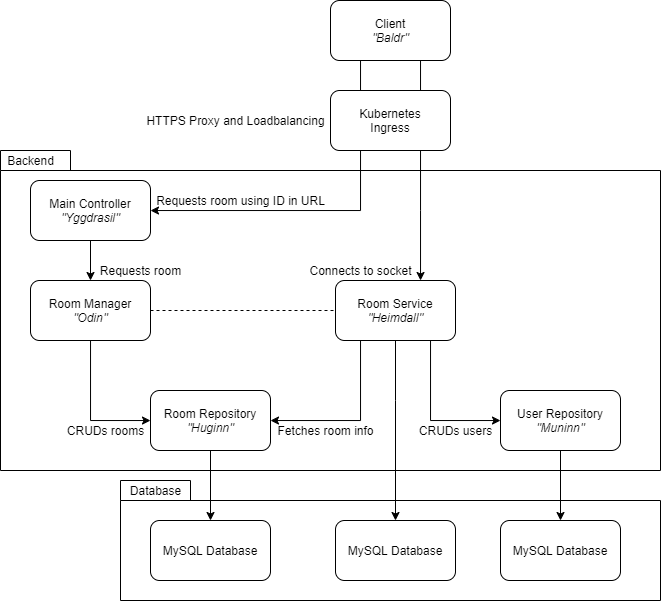
\includegraphics[width=\textwidth]{Pictures/Odin Final Design (3).png}
        \caption{The final Odin design. Larger version available here: \ref{fig:odinDesignFullSized}}
        \label{fig:odinfinaldesign}
    \end{subfigure}
    \hfill
    \begin{subfigure}[b]{0.48\textwidth}
        \centering
        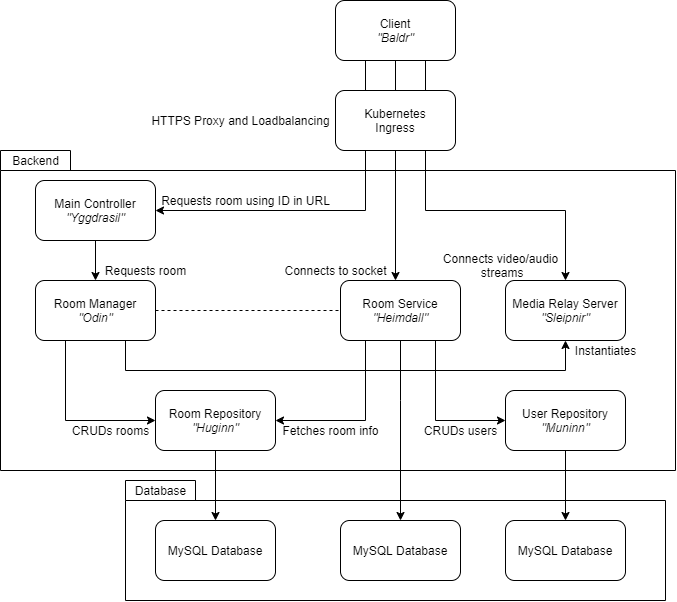
\includegraphics[width=\textwidth]{Pictures/Vili Final Design (4).png}
        \caption{The final Vili design. Larger version available here: \ref{fig:viliDesignFullSized}}
        \label{fig:vilifinaldesign}
    \end{subfigure}
    \caption{Block diagrams of twin designs of the Odin and Vili designs. It can be seen how the majority of components are identical, except for the use of the different room managers, as well as the addition of a Media Relay Server in the Vili design}
    \label{fig:finaldesigns}
\end{figure}

\subsection{The Twin Designs}

There are two designs for the system as shown in figure \ref{fig:finaldesigns}, one where voice and video communications are facilitated through P2P connections between clients, also known colloquially as the \textit{Odin design}, and one known colloquially as the \textit{Vili design} where voice and video communication is facilitated through a media relay server. These two designs are mostly identical in design, with most of the components shared between them. The room creator component is the major factor in each design\footnote{Vili never made it through to final implementation due to time constraints, but its influence remained.}, and as such is also where the names are derived from. The intent of the twin designs is to measure and compare their performances in accordance with the secondary project goal. The high level designs are shown in figures below.

Another major factor between the two designs is the WebRTC connections created between users. The P2P connection establishes a mesh connection between all other connected users, with all users having N-1 upstreams and N-1 down streams, N being user count. The media relay server (MRS) connection only allows users to have one upstream with the MRS. This stream is then shared between all other users connected. This would result in all users having 1 upstream and N-1 downstreams. An illustration of both of these implementations can be seen below \cite{webrtc-server}

\begin{figure}[ht]
    \centering
    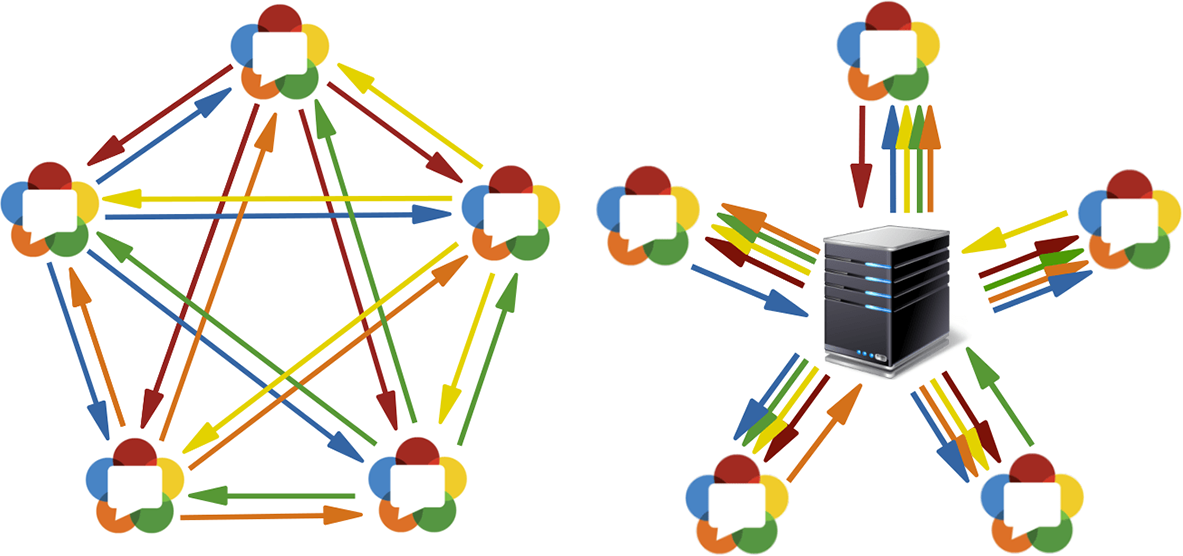
\includegraphics[width=\textwidth]{Pictures/webrtc-SFU-mesh.png}
    \caption{Two illustrations showing a Mesh P2P connection (Left) and SFU/MRS connection (right) courtesy of above citation.}
    \label{fig:gantt}
\end{figure}

\subsection{Major Components}

\subsubsection{Main Controller - Yggdrasil}

The Main Controller, nicknamed \textit{"Yggdrasil"}, is responsible for, as the name implies, connecting the worlds. Acting mostly as entry for the rest of the system, it is the service that the client first interacts with when requesting a room, and it is what returns the room client web page to the clients browser. It fetches the rooms requested from a room manager, and depending on the room manager implementation, will return different types of room behaviour to the user.

\subsubsection{Browser-based Client - Baldr}

The browser-based client, also known as \textit{"Baldr"} is what is returned to the client by Yggdrasil, and is what the client uses to login and interact with a room. It contains a number of sub components, including but not limited to one for connecting and interacting with the room server, one for connecting streams, and more.

\subsubsection{Room Service - Heimdall}

The service responsible for the rooms themselves is the one known as \textit{"Heimdall"}. It provides a socket endpoint for the client to connect to and listen for events from, as well as send information to, as well as a socket for sending signalling information between users. Heimdall is responsible for maintaining the many rooms and the users connected to them, as well as keeping the many rooms separated. It uses user- and room RESTful repository services in order to store information. Furthermore, it directly accesses its own database in order to store meta-information about the connected sockets.

\subsubsection{Room Managers - Odin and Vili}

The two room managers, known as \textit{"Odin"} and \textit{"Vili"}. These, upon request from Yggdrasil, returns room information which differs depending on which of the managers is in use. Odin merely returns the information needed for the client to connect to the room service Heimdall, while Vili does the same as well as instantiates an instance of the Media relay server for the client to connect to.

\subsubsection{Room and User Repositories - Huginn and Muninn}

The room and user repositories, respectively nicknamed \textit{"Huginn"} and \textit{"Muninn"}, are simple services which provide a RESTful API, in order to allow other services to easily perform CRUD operations on rooms and users, without each consuming service needing to implement its own database access.

\subsubsection{Media Relay Server - Sleipnir}

The Media Relay Server named \textit{"Sleipnir"} is as shown in figure \ref{fig:finaldesigns} entirely unique to the Vili design, and acts as a relay between clients for voice/video communication, by having the clients connect to Sleipnir, which then relays clients voice/video streams to each other.

\subsection{Major Changes Through Development}

Throughout development, the design endured a number of simplifying changes to an initial more complex design with unique service instances for each user and room, all managed by complex programmatic manipulation of the Kubernetes cluster the system was deployed on. The original designs, while intriguing, were deemed too impractical for implementation, and simplified to what is documented in this chapter. A block diagram of the initially proposed design is available as appendix \ref{fig:initialdesign1} and \ref{fig:initialdesign2}.

\subsection{Pros and Cons}

While the pros of a microservice-based design are clear in terms of scalability and reliability, there are however some significant cons with such a design. In particular as there is a significant development overhead in both complexity and labor needed to implement it. Following such a design poses limitations, such as the aforementioned statelessness and ephemeral nature, requiring further complexity when a component, for instance, need some sort of persistent storage. This is further discussed in the Evaluation and Reflections chapter.


\subsection{Merging the Twin Designs}

The possibility of merging the two designs into a single one, where the type of room would be selectable by the end-user, perhaps through a subscription or different endpoints, has been proposed and debated. The merging would in theory be simple, by merely adding support for accessing different room managers to Yggdrasil. However, it was deemed that this would likely lead to a number of unforeseen issues that would not be worth the trouble, and that time was better spent elsewhere.

\section{Conclusion}

The system architecture is for the vast majority of it based on microservice architecture principles, with the exception of a single component, which is closer to a client-server style architecture. The microservice-based architecture was chosen in particular for its scalability and good fit with containerization technologies. The design itself consists eight total components, used in two separate designs, which both share six central components. There are some additional parts to the design such as databases and a Kubernetes Ingress acting as a proxy and loadbalancer. The design has undergone a number of simplifying changes throughout development, as the initially proposed design was deemed too unfeasible and impractical to implement.